\documentclass[14pt]{beamer}
\usepackage{./Estilos/BeamerUVM}
\usepackage{./Estilos/ColoresLatex}
\usepackage{circuitikz}
\usepackage{schemata}
\usetheme{Warsaw}
\usecolortheme{rose}
%\useoutertheme{default}
\setbeamercovered{invisible}
% or whatever (possibly just delete it)
\setbeamertemplate{section in toc}[sections numbered]
\setbeamertemplate{subsection in toc}[subsections numbered]
\setbeamertemplate{subsection in toc}{\leavevmode\leftskip=3.2em\rlap{\hskip-2em\inserttocsectionnumber.\inserttocsubsectionnumber}\inserttocsubsection\par}
%\setbeamercolor{section in toc}{fg=blue}
%\setbeamercolor{subsection in toc}{fg=blue}
%\setbeamercolor{frametitle}{fg=blue}
\setbeamertemplate{caption}[numbered]

\setbeamertemplate{footline}
\beamertemplatenavigationsymbolsempty
\setbeamertemplate{headline}{}


\makeatletter
\setbeamercolor{section in foot}{bg=gray!30, fg=black!90!orange}
\setbeamercolor{subsection in foot}{bg=blue!30}
\setbeamercolor{date in foot}{bg=black}
\setbeamertemplate{footline}
{
  \leavevmode%
  \hbox{%
  \begin{beamercolorbox}[wd=.333333\paperwidth,ht=2.25ex,dp=1ex,center]{section in foot}%
    \usebeamerfont{section in foot} \insertsection
  \end{beamercolorbox}%
  \begin{beamercolorbox}[wd=.333333\paperwidth,ht=2.25ex,dp=1ex,center]{subsection in foot}%
    \usebeamerfont{subsection in foot}  \insertsubsection
  \end{beamercolorbox}%
  \begin{beamercolorbox}[wd=.333333\paperwidth,ht=2.25ex,dp=1ex,right]{date in head/foot}%
    \usebeamerfont{date in head/foot} \hspace*{2em}
    \insertframenumber{} / \inserttotalframenumber \hspace*{2ex} 
  \end{beamercolorbox}}%
  \vskip0pt%
}
\makeatother

\makeatletter
\patchcmd{\beamer@sectionintoc}{\vskip1.5em}{\vskip0.8em}{}{}
\makeatother
% \usefonttheme{serif}
\usepackage[clock]{ifsym}
\DeclareSIUnit\erg{erg}
\DeclareSIUnit[number-unit-product = {\,}]\cal{cal}

\sisetup{per-mode=symbol}
\resetcounteronoverlays{saveenumi}

% Macro para agregar el logo de UVM en cada slide de la presentación

\addtobeamertemplate{frametitle}{}{%
\begin{tikzpicture}[remember picture,overlay]
\coordinate (logo) at ([xshift=-1.5cm,yshift=-0.8cm]current page.north east);
% \fill[devryblue] (logo) circle (.9cm);
% \clip (logo) circle (.75cm);
\node at (logo) {
\includegraphics[width=2.1cm]{Imagenes/logo_UVM.png}};
\end{tikzpicture}}


\title{\Large{Instrumentación biomédica I} \\ \normalsize{Física IV (Área II)}}
\date{}

\begin{document}
\maketitle

\section*{Contenido}
\frame[allowframebreaks]{\frametitle{Contenido} \tableofcontents[currentsection, hideallsubsections]}

\section{Instrumentación}
\frame{\tableofcontents[currentsection, hideothersubsections]}
\subsection{Estetoscopio}

\begin{frame}
\frametitle{El estestoscopio}
El \textocolor{ao}{estetoscopio} es un \textocolor{awesome}{dispositivo acústico} que amplifica los ruidos corporales para lograr su mejor percepción.
\end{frame}
\begin{frame}
\frametitle{El estestoscopio}
Favorece la integración de diversos signos, \pause los cuales se auscultan principalmente en corazón, pulmones y abdomen.
\end{frame}
\begin{frame}
\frametitle{¿Qué es un signo?}
Es algo que se \textocolor{brown(web)}{identifica durante un examen físico}, \pause \textocolor{brown(web)}{una prueba de laboratorio} \pause o \textocolor{brown(web)}{una prueba con imágenes} \pause que indica la posibilidad de que una persona tenga una afección o enfermedad.
\end{frame}
\begin{frame}
\frametitle{¿Qué es un signo?}
Los signos los pueden observar un profesional de atención de la salud u otra persona.
\end{frame}
\begin{frame}
\frametitle{¿Qué es un signo?}
Algunos ejemplos son la fiebre, la inflamación, el sarpullido, la presión arterial alta o la glucemia alta.
\end{frame}
\begin{frame}
\frametitle{¿Qué es un síntoma?}
Algo que \textocolor{armygreen}{una persona siente o experimenta} y que tal vez indique una enfermedad o afección.
\end{frame}
\begin{frame}
\frametitle{¿Qué es un síntoma?}
Los síntomas solo los puede notificar la persona que los presenta, \pause no los observa el proveedor de atención de la salud y no se manifiestan en los exámenes médicos.
\end{frame}
\begin{frame}
\frametitle{¿Qué es un síntoma?}
Algunos ejemplos de síntomas son el dolor, las náuseas, la fatiga y la ansiedad.
\end{frame}
\begin{frame}
\frametitle{Tipos de estetoscopios}
\schema
    {
        \schemabox{Estestoscopios}
    }
    {
        \schemabox{Electrónicos \\ \\
                \schema
                        {
                            \schemabox{Auditivos/Mecánicos}
                        } 
                        {
                            \schemabox{Pinard \\ \\ Biauricular}
                        }
    }}
\end{frame}
\begin{frame}
\frametitle{Estetoscopio de Pinard}
Son usados exclusivamente para la auscultación de latidos cardíacos fetales.
\end{frame}
\begin{frame}
\frametitle{Estetoscopio de Pinard}
\begin{figure}
    \centering
    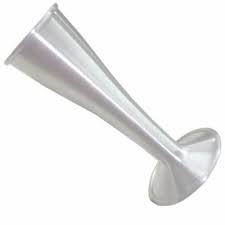
\includegraphics[scale=0.75]{Imagenes/Estetoscopio_01.jpg}
\end{figure}
\end{frame}
\begin{frame}
\frametitle{Estetoscopio de Pinard}
La principal \textocolor{red}{diferencia} entre un estetoscopio de Pinard y un convencional \pause es que se puede escuchar el latido fetal de forma directa.
\end{frame}
\begin{frame}
\frametitle{Estetoscopio de Pinard}
Ya que en el estetoscopio Pinard el sonido pasa directamente del vientre materno al oído del auscultante.
\end{frame}
\begin{frame}
\frametitle{Estetoscopio de Pinard}
\vspace*{-1cm}
\begin{figure}
    \centering
    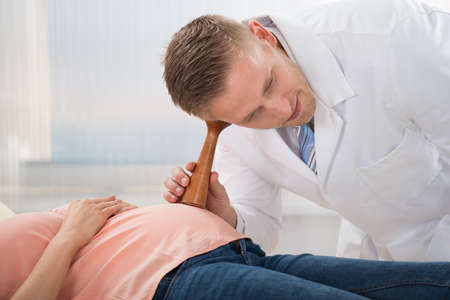
\includegraphics[scale=0.5]{Imagenes/Estetoscopio_02.jpg}
\end{figure}
\end{frame}
\begin{frame}
\frametitle{Estetoscopio Biauricular}
Los estetoscopios están conformados por las siguientes partes que, en conjunto, \pause \textocolor{bole}{transfieren la información acústica} desde la superficie corporal hasta los oídos del examinador.
\end{frame}
\begin{frame}
\frametitle{Pieza corporal o cabeza}
Su función es \textocolor{lava}{captar y amplificar} los ruidos corporales de diferentes frecuencias (de 125 Hz a 3000 Hz).
\end{frame}
\begin{frame}
\frametitle{Pieza corporal o cabeza}
Existen dos tipos de cápsulas.
\pause
\setbeamercolor{item projected}{bg=bananayellow,fg=ao}
\setbeamertemplate{enumerate items}{%
\usebeamercolor[bg]{item projected}%
\raisebox{1.5pt}{\colorbox{bg}{\color{fg}\footnotesize\insertenumlabel}}%
}
\begin{enumerate}[<+->]
\item \textocolor{carmine}{Cápsula de Campana.}

De forma cónica circular y con un arillo de plástico semirrígido en el borde exterior.
\seti
\end{enumerate}
\end{frame}
\begin{frame}
\frametitle{Pieza corporal o cabeza}
\setbeamercolor{item projected}{bg=bananayellow,fg=ao}
\setbeamertemplate{enumerate items}{%
\usebeamercolor[bg]{item projected}%
\raisebox{1.5pt}{\colorbox{bg}{\color{fg}\footnotesize\insertenumlabel}}%
}
\begin{enumerate}[<+->]
\conti
\item \textocolor{carmine}{Cápsula con Diafragma.}

La cápsula es de metal (acero inoxidable, bronce cromado o titanio), de forma circular y sus dimensiones están relacionadas con las del diafragma.
\end{enumerate}
\end{frame}
\begin{frame}
\frametitle{Partes del estetoscopio}
\vspace*{-1cm}
\begin{figure}
    \centering
    
\includegraphics[scale=0.7]{Imagenes/Estetoscopio_03.png}
\end{figure}
\end{frame}
\begin{frame}
\frametitle{Por tipo de cápsula}
Los estetoscopios se dividen principalmente en dos tipos, dependiendo del tipo
de cápsulas:
\pause
\setbeamercolor{item projected}{bg=classicrose,fg=black}
\setbeamertemplate{enumerate items}{%
\usebeamercolor[bg]{item projected}%
\raisebox{1.5pt}{\colorbox{bg}{\color{fg}\footnotesize\insertenumlabel}}%
}
\begin{enumerate}[<+->]
\item \textbf{Sencillo.}

Solamente cuenta con una cápsula de diafragma y debe detener un vástago fijo para su unión con el tubo flexible.
\conti
\end{enumerate}
\end{frame}
\begin{frame}
\frametitle{Por tipo de cápsula}
\setbeamercolor{item projected}{bg=classicrose,fg=black}
\setbeamertemplate{enumerate items}{%
\usebeamercolor[bg]{item projected}%
\raisebox{1.5pt}{\colorbox{bg}{\color{fg}\footnotesize\insertenumlabel}}%
}
\begin{enumerate}[<+->]
\conti
\item \textbf{Múltiple.}

Pueden ser de dos o más cápsulas. Deben de tener una válvula selectora fija, que permita seleccionar y operar sólo una de las cápsulas.    
\end{enumerate}
\end{frame}
\begin{frame}
\frametitle{Tubo flexible}
Este tubo usualmente es de PVC, plástico o de hule flexible, \pause pudiendo ser sencillo (de una sola pieza) en su porción de la pieza pectoral hasta la división donde se dirige a cada uno de los tubos metálicos auriculares (en forma de \enquote{Y})
\end{frame}
\begin{frame}
\frametitle{Tubo flexible}
En esta zona se reduce su calibre \pause esto obviamente en detrimento de la calidad acústica del sonido que se percibe.
\end{frame}
\begin{frame}
\frametitle{Tubo flexible}
Debe de tener un diámetro interior mínimo de 4.0 mm y una longitud mínima de 50 cm a partir de la parte final de la \enquote{Y}.
\end{frame}
\begin{frame}
\frametitle{Partes del estetoscopio}
\vspace*{-1cm}
\begin{figure}
    \centering
    
\includegraphics[scale=0.7]{Imagenes/Estetoscopio_04.png}
\end{figure}
\end{frame}
\begin{frame}
\frametitle{Muelle}
El \textocolor{blue-violet}{muelle es de acero inoxidable}, bronce cromado o titanio.
\end{frame}
\begin{frame}
\frametitle{Tubos auditivos}
Los tubos auditivos deben de tener roscas, estrías o algún diseño adecuado para \textocolor{cardinal}{asegurar el correcto ensamble} con las olivas, el tubo flexible y el muelle.
\end{frame}
\begin{frame}
\frametitle{Partes del estetoscopio}
\vspace*{-1cm}
\begin{figure}
    \centering
    
\includegraphics[scale=0.7]{Imagenes/Estetoscopio_05.png}
\end{figure}
\end{frame}
\begin{frame}
\frametitle{Olivas}
Estas pueden ser de material suave o rígido, siendo más cómodas las de material suave.
\end{frame}
\begin{frame}
\frametitle{Olivas}
Las olivas de material rígido ofrecen un sello más hermético y por tanto una mejor transmisión acústica.
\end{frame}
\begin{frame}
\frametitle{Partes del estetoscopio}
\vspace*{-1cm}
\begin{figure}
    \centering
    
\includegraphics[scale=0.7]{Imagenes/Estetoscopio_06.png}
\end{figure}
\end{frame}

\subsection{Esfigmomanómetro}

\begin{frame}
\frametitle{¿Qué es el esfigmomanómetro?}
Ee un equipo auxiliar de diagnóstico empleado para la \textocolor{ceruleanblue}{medición no invasiva o indirecta de la presión arterial}.
\end{frame}
\begin{frame}
\frametitle{Tipos de esfigmomanómetro}
\schema
    {
        \schemabox{Esfigmomanómetros}
    }
    {
        \schemabox{Mercurial \\ \\ Aneroide \\ \\ Electrónico}
    }
\end{frame}

\begin{frame}
\frametitle{Parte del esfigmomanómetro}
Consta de un \textocolor{crimsonglory}{brazalete inflable}, \pause \textocolor{darkred}{una perilla} para inflarlo y \pause \textocolor{debianred}{un medidor de presión} que puede ser de columna de mercurio, aneroide o electrónico.
\end{frame}
\begin{frame}
\frametitle{El esfigmomanómetro mercurial}
\vspace*{-1cm}
\begin{figure}
    \centering
    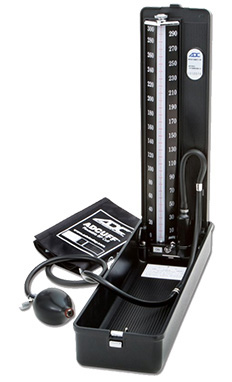
\includegraphics[scale=0.45]{Imagenes/Esfigmomanometro_01.jpg}
\end{figure}
\end{frame}
\begin{frame}
\frametitle{¿Para qué se usa?}
El método más utilizado para conocer el valor de la presión arterial, presión que ejerce la sangre sobre las paredes de las arterias, es mediante la técnica auscultatoria.
\end{frame}
\begin{frame}
\frametitle{El esfigmomanómetro}
\vspace*{-1cm}
\begin{figure}
    \centering
    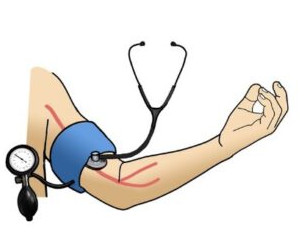
\includegraphics[scale=2]{Imagenes/Esfigmomanometro_02.jpg}
\end{figure}
\end{frame}
\begin{frame}
\frametitle{¿Qué se registra?}
Durante estos procedimientos, se determinan:
\pause
\setbeamercolor{item projected}{bg=eggplant,fg=white}
\setbeamertemplate{enumerate items}{%
\usebeamercolor[bg]{item projected}%
\raisebox{1.5pt}{\colorbox{bg}{\color{fg}\footnotesize\insertenumlabel}}%
}
\begin{enumerate}[<+->]
\item \textocolor{red}{Presión sistólica}.

Es la que ejerce el flujo sanguíneo sobre las arterias cuando los músculos del corazón se contraen.
\seti
\end{enumerate}
\end{frame}
\begin{frame}
\frametitle{¿Qué se registra?}
Durante estos procedimientos, se determinan:
\pause
\setbeamercolor{item projected}{bg=eggplant,fg=white}
\setbeamertemplate{enumerate items}{%
\usebeamercolor[bg]{item projected}%
\raisebox{1.5pt}{\colorbox{bg}{\color{fg}\footnotesize\insertenumlabel}}%
}
\begin{enumerate}[<+->]
\conti
\item \textocolor{red}{Presión diastólica}.

Es la que ejerce el flujo sanguíneo sobre las arterias entre dos contracciones cardiacas.
\end{enumerate}
\end{frame}
\begin{frame}
\frametitle{Principio de operación}
El procedimiento para la toma de la presión arterial se fundamenta en la \textocolor{ao}{auscultación de sonidos} (\textocolor{falured}{ruidos de Korotkoff}) \pause que se generan en las arterias periféricas (normalmente la arteria radial) cuando \textocolor{electricviolet}{se modifica el flujo de la sangre}.
\end{frame}
\begin{frame}
\frametitle{Los ruidos de Korotkoff}
Los \textocolor{falured}{ruidos de Korotkoff} fueron descritos desde 1905 y se describieron 5 fases.
\end{frame}
\begin{frame}
\frametitle{Los ruidos de Korotkoff}
Cuando el brazalete alrededor del brazo se infla con una presión mayor a la presión sistólica no se escucha nada debido a que se ocluye la arteria evitando el flujo.
\end{frame}
\begin{frame}
\frametitle{Los ruidos de Korotkoff}
Conforme va disminuyendo la presión y se permite gradualmente un mayor paso de sangre a través de la zona de oclusión se pueden observar las siguientes fases:
\end{frame}
\begin{frame}
\frametitle{Los ruidos de Korotkoff}
\setbeamercolor{item projected}{bg=goldenpoppy,fg=black}
\setbeamertemplate{enumerate items}{%
\usebeamercolor[bg]{item projected}%
\raisebox{1.5pt}{\colorbox{bg}{\color{fg}\footnotesize\insertenumlabel}}%
}
\begin{enumerate}[<+->]
\item \textocolor{indigo(web)}{Primera:} es un sonido más fuerte y agudo, el primero en escucharse cuando la presión sistólica es mayor que la presión del brazalete.
\seti
\end{enumerate}
\end{frame}
\begin{frame}
\frametitle{Los ruidos de Korotkoff}
\setbeamercolor{item projected}{bg=goldenpoppy,fg=black}
\setbeamertemplate{enumerate items}{%
\usebeamercolor[bg]{item projected}%
\raisebox{1.5pt}{\colorbox{bg}{\color{fg}\footnotesize\insertenumlabel}}%
}
\begin{enumerate}[<+->]
\conti
\item \textocolor{indigo(web)}{Segunda:} son murmullos oídos en la mayor parte del tiempo entre la primera y las últimas fases (entre los valores de las presiones sistólicas y diastólicas).
\seti
\end{enumerate}
\end{frame}
\begin{frame}
\frametitle{Los ruidos de Korotkoff}
\setbeamercolor{item projected}{bg=goldenpoppy,fg=black}
\setbeamertemplate{enumerate items}{%
\usebeamercolor[bg]{item projected}%
\raisebox{1.5pt}{\colorbox{bg}{\color{fg}\footnotesize\insertenumlabel}}%
}
\begin{enumerate}[<+->]
\conti
\item \textocolor{indigo(web)}{Tercera y cuarta fases:} se oyen en presiones aproximadamente de 10 mmHg por arriba de la presión sanguínea diastólica, descritos ambos como \enquote{golpeando pesadamente} y \enquote{amortiguados}.
\seti
\end{enumerate}
\end{frame}
\begin{frame}
\frametitle{Los ruidos de Korotkoff}
\setbeamercolor{item projected}{bg=goldenpoppy,fg=black}
\setbeamertemplate{enumerate items}{%
\usebeamercolor[bg]{item projected}%
\raisebox{1.5pt}{\colorbox{bg}{\color{fg}\footnotesize\insertenumlabel}}%
}
\begin{enumerate}[<+->]
\conti
\item \textocolor{indigo(web)}{Quinta fase:} es el silencio que se oye a medida que la presión del brazalete cae debajo de la presión sanguínea diastólica.
\end{enumerate}
\end{frame}
\begin{frame}
\frametitle{Los ruidos de Korotkoff}
Aunque tradicionalmente se tomaba para determinar la presión diastólica el punto en que el cuarto ruido se escucha muy tenuemente.
\end{frame}
\begin{frame}
\frametitle{Los ruidos de Korotkoff}
Actualmente se prefiere usar la quinta fase (silencio) para determinar el valor de la presión diastólica.
\end{frame}
\begin{frame}
\frametitle{El esfigmomanómetro}
\vspace*{-1cm}
\begin{figure}
    \centering
    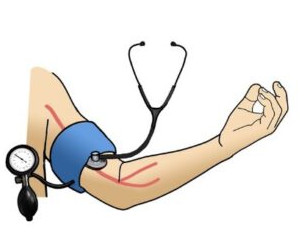
\includegraphics[scale=2]{Imagenes/Esfigmomanometro_02.jpg}
\end{figure}
\end{frame}
\begin{frame}
\frametitle{La auscultación}
\vspace*{-1cm}
\begin{figure}
    \centering
    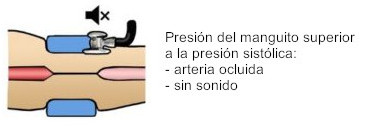
\includegraphics[scale=2]{Imagenes/Esfigmomanometro_03.jpg}
\end{figure}
\end{frame}
\begin{frame}
\frametitle{La auscultación}
\vspace*{-1cm}
\begin{figure}
    \centering
    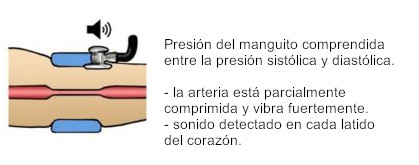
\includegraphics[scale=2]{Imagenes/Esfigmomanometro_04.jpg}
\end{figure}
\end{frame}
\begin{frame}
\frametitle{La auscultación}
\vspace*{-1cm}
\begin{figure}
    \centering
    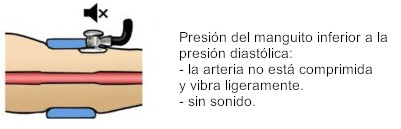
\includegraphics[scale=2]{Imagenes/Esfigmomanometro_05.jpg}
\end{figure}
\end{frame}
\begin{frame}
\frametitle{¿Por qué se generan los ruidos?}
Tiene que ver con el \textocolor{red}{cambio} de un \textocolor{lincolngreen}{flujo laminar} a un \textocolor{magenta}{flujo turbulento}.
\end{frame}
\begin{frame}
\frametitle{Flujo laminar de la sangre}
En una arteria normal, las paredes son lo suficientemente lisas para que la sangre tenga un \textocolor{lincolngreen}{flujo laminar} en un patrón ordenado.
\end{frame}
\begin{frame}
\frametitle{Flujo laminar de la sangre}
Las moléculas de la sangre pegadas a las paredes arteriales prácticamente no se mueven y las partículas en el centro de la arteria tienen la máxima velocidad de movimiento.
\end{frame}
\begin{frame}
\frametitle{Flujo turbulento de la sangre}
Cuando existe \textocolor{pansypurple}{un obstáculo} como un coágulo, un ateroma, o las paredes de la
arteria al ser comprimida por el brazalete del esfigmomanómetro, etc.
\end{frame}
\begin{frame}
\frametitle{Flujo turbulento de la sangre}
El \textocolor{lincolngreen}{flujo laminar} se distorsiona y se vuelve \textocolor{magenta}{flujo turbulento}, \pause  algunas moléculas de sangre empiezan a fluir en direcciones axiales y se mezclan.
\end{frame}
\begin{frame}
\frametitle{Los ruidos de Korotkoff}
\vspace*{-1cm}
\begin{figure}
    \centering
    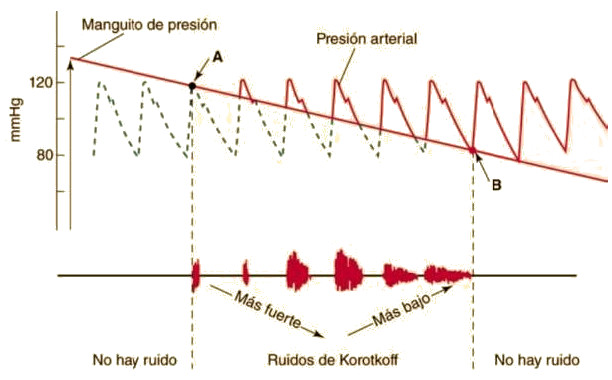
\includegraphics[scale=0.6]{Imagenes/Esfigmomanometro_06.jpg}
\end{figure}
\end{frame}     
\begin{frame}
\frametitle{Esfigmomanómetro aneroide}
Este dispositivo tiene las mismas características del mercurial pero en lugar de un manómetro de mercurio utiliza un mecanismo aneroide, lo que lo hace más ligero y transportable.
\end{frame}
\begin{frame}
\frametitle{Esfigmomanómetro aneroide}
\vspace*{-1cm}
\begin{figure}
    \centering
    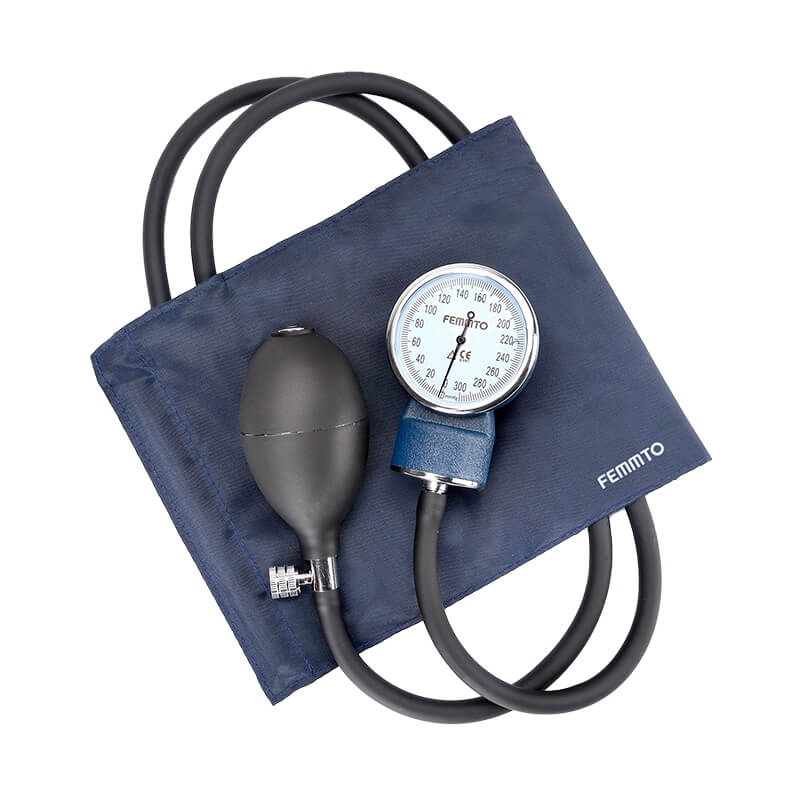
\includegraphics[scale=0.25]{Imagenes/Esfigmomanometro_07.jpg}
\end{figure}
\end{frame}
\begin{frame}
\frametitle{Esfingomanómetro electrónico}
Pueden ser semi-automáticos o automáticos, ambos incluyen un sensor de presión y una pantalla digital.
\end{frame}
\begin{frame}
\frametitle{Esfigmomanómetro electrónico}
\vspace*{-1cm}
\begin{figure}
    \centering
    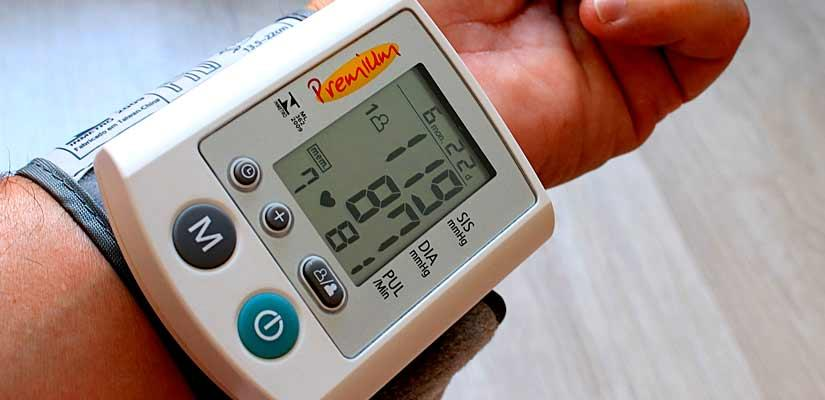
\includegraphics[scale=0.35]{Imagenes/Esfigmomanometro_08.jpg}
\end{figure}
\end{frame}
\end{document}